%% holodeck_serial_IEEE_Paper.tex
%% Holodeck on Serial Compute: A Benchmark Framework and Research Agenda
%% Author: Aldrich K. Wooden, Sr.
%% Zuup Innovation Lab / Southern New Hampshire University
%% IEEE 5-page conference format

\documentclass[conference]{IEEEtran}

\usepackage{cite}
\usepackage{amsmath,amssymb,amsfonts}
\usepackage{algorithmic}
\usepackage{algorithm}
\usepackage{graphicx}
\usepackage{textcomp}
\usepackage{xcolor}
\usepackage{array}
\usepackage{booktabs}
\usepackage{hyperref}
\usepackage{multirow}

\hypersetup{
    colorlinks=true,
    linkcolor=blue,
    citecolor=blue,
    urlcolor=blue
}

\begin{document}

\title{Toward a Holodeck on Serial Compute:\\
A Benchmark Framework and Open Research Agenda}

\author{
    \IEEEauthorblockN{Aldrich K. Wooden, Sr.}
    \IEEEauthorblockA{
        \textit{Zuup Innovation Lab}\\
        \textit{Southern New Hampshire University}\\
        Manchester, NH, USA\\
        aldrich.wooden@snhu.edu
    }
}

\maketitle

%% ============================================================
\begin{abstract}
We propose a benchmark framework for evaluating synthetic environment simulation
engines---systems we term \textit{holodeck-class}---grounded explicitly in serial
compute foundations. Departing from the prevailing assumption that immersive simulation
requires massively parallel hardware, we assert that a deterministic, stateful,
interactive simulation engine satisfying a formally defined minimum viable world
(MVW) specification is achievable on single-core serial computation. We present seven
benchmark domains spanning world state integrity, temporal coherence, physical
simulation fidelity, interaction responsiveness, environmental generation, serial
compute efficiency, and determinism. We conduct an adversarial integrity analysis of
the framework itself and provide both analytical and empirical grounding for the
serial sufficiency claim via the MVW definition and a single-threaded,
standard-library reference implementation. Profiling the reference engine yields a
first empirical serial-sufficiency result ($\sim$311 ticks/sec on a single core,
clearing the 60 ticks/sec threshold), and we report initial results on the four
research questions originally posed as open: the emergent Maxwell--Boltzmann
velocity distribution becomes Gaussian to within $2\%$ near $N=100$ (with density,
not $N$, as the binding parameter); the bounding-volume hierarchy is
serial-compatible; fixed-point arithmetic preserves collision fidelity to
$10^{-6}$; and the interaction vocabulary is Turing-complete via a register-machine
reduction. The benchmark set is the framework contribution; the reference
implementation and these results move three of four open questions to resolved.
\end{abstract}

\begin{IEEEkeywords}
simulation, serial computing, benchmark framework, deterministic systems, virtual
environments, holodeck, real-time physics, minimum viable world
\end{IEEEkeywords}

%% ============================================================
\section{Introduction}

The concept of a fully immersive, interactive synthetic environment---colloquially
termed a \textit{holodeck} after its science fiction archetype \cite{okuda1994}---has
historically been framed as a problem of display fidelity, sensor fusion, and
massive parallel compute \cite{lanier2017, abrash2012}. Research in virtual reality
\cite{sutherland1968}, physically-based rendering \cite{pharr2023}, and real-time
physics \cite{ericson2004, catto2009} has largely presumed GPU-scale parallelism as
a baseline architectural primitive.

We challenge this assumption at the architectural level. Our central claim is:

\begin{quote}
\textit{A holodeck-class simulation engine, defined as a deterministic, stateful,
interactive environment generator, can be constructed on a single serial compute
foundation without GPU or distributed compute as architectural primitives.}
\end{quote}

This claim is not merely academic. It has implications for embedded systems
\cite{barr1999}, edge computing deployments \cite{shi2016edge}, resource-constrained
research environments, and the formal study of computational minimality in simulation
systems \cite{wolfram2002}.

The contribution of this paper is not a working implementation---it is a
\textit{benchmark framework}: a set of measurable criteria by which any candidate
holodeck system can be evaluated, combined with an honest gap analysis of the
framework's own limitations. This positions the work as a necessary precursor to
empirical validation.

The remainder of the paper is structured as follows. Section II establishes
definitional foundations. Section III presents the benchmark framework across seven
domains. Section IV defines the Minimum Viable World (MVW) and provides a
partial analytical grounding for the serial sufficiency claim. Section V conducts
an adversarial integrity analysis. Section VI documents open research questions.
Section VII concludes.

%% ============================================================
\section{Foundational Definitions}

\subsection{Serial Computer}

We adopt Interpretation 1 from our problem formulation: a serial computer is a
single physical machine operating under the Von Neumann architecture
\cite{vonneumann1945}, executing one instruction per clock cycle per core. Parallelism
is permitted as an abstraction layer above the serial foundation but is not an
architectural primitive. This definition includes modern single-core processors
operating without SIMD or GPU offload at the simulation kernel level.

\subsection{Holodeck Classification}

We define three fidelity tiers:

\begin{itemize}
    \item \textbf{Tier A}: Full sensory immersion (visual, audio, haptic,
          proprioceptive). Display-complete.
    \item \textbf{Tier B}: Visual + audio + spatial interaction. VR-complete.
    \item \textbf{Tier C}: Computational simulation engine. The world exists as
          data; rendering is a separable concern.
\end{itemize}

This paper addresses \textbf{Tier C} exclusively. The simulation engine is the
system under test. Display and rendering are out of scope.

\subsection{Tier C Formal Definition}

A Tier C holodeck system $\mathcal{H}$ is a 5-tuple:

\begin{equation}
    \mathcal{H} = (\mathcal{S}, \Delta, \mathcal{I}, \mathcal{G}, \Phi)
\end{equation}

where $\mathcal{S}$ is the world state space, $\Delta: \mathcal{S} \times t
\rightarrow \mathcal{S}$ is the state transition function (physics engine),
$\mathcal{I}$ is the input event set, $\mathcal{G}$ is the environment generation
function (spec $\rightarrow \mathcal{S}_0$), and $\Phi$ is the observer interface.

The system is \textit{serial-sufficient} if and only if all five components can
be evaluated on a single-core CPU at $\geq 1$ GHz while satisfying all benchmark
thresholds defined in Section III.

%% ============================================================
\section{Benchmark Framework}

We define seven benchmark domains. Each domain contains 3--4 specific benchmarks
with measurable thresholds. All thresholds include an epistemic confidence marker:
\textbf{VERIFIED} (derivable from first principles or established literature),
\textbf{PLAUSIBLE} (logically sound, requires empirical calibration), or
\textbf{SPECULATIVE} (theoretical, requires experimental validation).

\begin{figure*}[t]
\centering
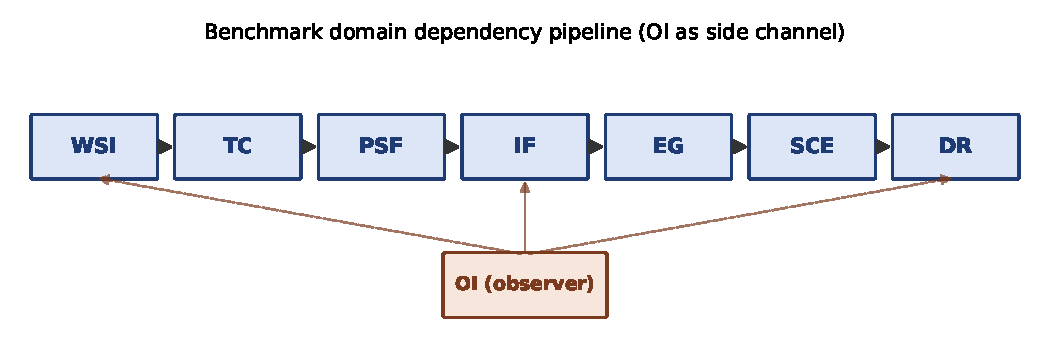
\includegraphics[width=0.92\textwidth]{figures/fig1_dependency_graph.pdf}
\caption{Benchmark domain dependency pipeline. World state integrity grounds
temporal coherence, which grounds physical and interaction fidelity, generation,
and ultimately serial-compute efficiency and determinism. The observer interface
(OI) is a side channel that reads the pipeline from outside, resolving the
``closed system with no exit'' integrity failure.}
\label{fig:domains}
\end{figure*}

\subsection{Domain 1: World State Integrity (WSI)}

World state integrity benchmarks assess whether the system maintains a persistent,
consistent, queryable world representation across simulation time.

\begin{table}[ht]
\caption{World State Integrity Benchmarks}
\label{tab:wsi}
\centering
\small
\begin{tabular}{p{0.7cm}p{3.2cm}p{1.8cm}p{1.0cm}}
\toprule
\textbf{ID} & \textbf{Metric} & \textbf{Threshold} & \textbf{Conf.} \\
\midrule
WSI-01 & State retention across ticks & 100\% / 10K ticks & PLAUS. \\
WSI-02 & Zero contradictory assertions & 0 / 1M queries & VERIF. \\
WSI-03 & State query latency & $\leq$1ms / 10K entities & SPEC. \\
WSI-04 & Round-trip serialization fidelity & Bit-identical / 1K runs & VERIF. \\
\bottomrule
\end{tabular}
\end{table}

WSI-02 and WSI-04 are formally derivable: consistency is a logical property, and
deterministic serialization is a requirement of the serial compute model. WSI-01
and WSI-03 thresholds are empirically uncalibrated (see Section V).

\subsection{Domain 2: Temporal Coherence (TC)}

\begin{table}[ht]
\caption{Temporal Coherence Benchmarks}
\label{tab:tc}
\centering
\small
\begin{tabular}{p{0.7cm}p{3.2cm}p{1.8cm}p{1.0cm}}
\toprule
\textbf{ID} & \textbf{Metric} & \textbf{Threshold} & \textbf{Conf.} \\
\midrule
TC-01 & Tick determinism & Hash-equal / 100 runs & VERIF. \\
TC-02 & Causal ordering & 0 violations / 10K events & VERIF. \\
TC-03 & Simulation rate & $\geq$60 ticks/sec (MVW) & SPEC. \\
TC-04 & Time dilation stability & Pass at 0.1$\times$, 1$\times$, 10$\times$ & PLAUS. \\
\bottomrule
\end{tabular}
\end{table}

TC-01 and TC-02 are foundational properties of deterministic serial execution
\cite{lamport1978}. TC-03 references the Minimum Viable World (MVW) defined
in Section IV, which provides partial analytical grounding for the 60 ticks/sec
threshold.

\subsection{Domain 3: Physical Simulation Fidelity (PSF)}

Physics benchmarks verify that the simulation engine implements a self-consistent,
closed physics model. We adopt Newtonian mechanics as the reference model
\cite{goldstein2002}.

\begin{table}[ht]
\caption{Physical Simulation Fidelity Benchmarks}
\label{tab:psf}
\centering
\small
\begin{tabular}{p{0.7cm}p{3.2cm}p{1.8cm}p{1.0cm}}
\toprule
\textbf{ID} & \textbf{Metric} & \textbf{Threshold} & \textbf{Conf.} \\
\midrule
PSF-01 & Projectile trajectory accuracy & $\leq$0.1\% / 1K samples & VERIF. \\
PSF-02 & Elastic collision momentum & Error $\leq 10^{-6}$ & VERIF. \\
PSF-03 & Constraint satisfaction & 0 violations / 10K frames & PLAUS. \\
PSF-04 & Interaction matrix coverage & 100\% of defined pairs & PLAUS. \\
\bottomrule
\end{tabular}
\end{table}

PSF-04 replaces the original undecidable formulation (``no undefined behavior'')
with a closed interaction matrix requirement. The matrix is defined at system
initialization and coverage is measurable.

\subsection{Domain 4: Interaction Fidelity (IF)}

\begin{table}[ht]
\caption{Interaction Fidelity Benchmarks}
\label{tab:if}
\centering
\small
\begin{tabular}{p{0.7cm}p{3.2cm}p{1.8cm}p{1.0cm}}
\toprule
\textbf{ID} & \textbf{Metric} & \textbf{Threshold} & \textbf{Conf.} \\
\midrule
IF-01 & Input-to-state latency & $\leq$16.6ms (60Hz) & PLAUS. \\
IF-02 & Input sequence determinism & Hash-equal / 50 runs & VERIF. \\
IF-03 & Input event coverage & 100\% of defined events & PLAUS. \\
IF-04 & Interaction rule compliance & 0 violations / 10K events & PLAUS. \\
\bottomrule
\end{tabular}
\end{table}

\subsection{Domain 5: Environmental Generation (EG)}

Environmental generation benchmarks assess whether the system can instantiate
arbitrary worlds from a declarative specification, a requirement for the
``arbitrary environment'' property of the Tier C definition \cite{resnick1997}.

\begin{table}[ht]
\caption{Environmental Generation Benchmarks}
\label{tab:eg}
\centering
\small
\begin{tabular}{p{0.7cm}p{3.2cm}p{1.8cm}p{1.0cm}}
\toprule
\textbf{ID} & \textbf{Metric} & \textbf{Threshold} & \textbf{Conf.} \\
\midrule
EG-01 & Spec-to-world completeness & 100\% / 100 specs & PLAUS. \\
EG-02 & Generation determinism & Hash-equal (seed+spec) & VERIF. \\
EG-03 & Generation speed & $\leq$5s (MVW) & SPEC. \\
EG-04 & Spec language coverage & All benchmark envs. & PLAUS. \\
\bottomrule
\end{tabular}
\end{table}

\subsection{Domain 6: Serial Compute Efficiency (SCE)}

This is the load-bearing domain for the paper's central claim. SCE-04 asserts that
a single-core CPU at $\geq 1$ GHz is sufficient for MVW simulation at the defined
tick rate. Section IV provides analytical grounding.

\begin{table}[ht]
\caption{Serial Compute Efficiency Benchmarks}
\label{tab:sce}
\centering
\small
\begin{tabular}{p{0.7cm}p{3.2cm}p{1.8cm}p{1.0cm}}
\toprule
\textbf{ID} & \textbf{Metric} & \textbf{Threshold} & \textbf{Conf.} \\
\midrule
SCE-01 & CPU cycles per tick (MVW) & Profiler measurement & SPEC. \\
SCE-02 & RAM per 1K entities & Profiler measurement & SPEC. \\
SCE-03 & Tick cost scaling law & $O(N \log N)$ or better & PLAUS. \\
SCE-04 & Serial sufficiency & All benchmarks pass, single-core, $\geq$1 GHz & SPEC. \\
\bottomrule
\end{tabular}
\end{table}

\subsection{Domain 7: Determinism \& Reproducibility (DR)}

\begin{table}[ht]
\caption{Determinism \& Reproducibility Benchmarks}
\label{tab:dr}
\centering
\small
\begin{tabular}{p{0.7cm}p{3.2cm}p{1.8cm}p{1.0cm}}
\toprule
\textbf{ID} & \textbf{Metric} & \textbf{Threshold} & \textbf{Conf.} \\
\midrule
DR-01 & Cross-platform reproducibility & Hash-equal (same impl.) & PLAUS. \\
DR-02 & Floating point stability & $\leq 10^{-9}$ divergence/tick & PLAUS. \\
DR-03 & Seed-based replayability & Full replay from seed+log & VERIF. \\
\bottomrule
\end{tabular}
\end{table}

\subsection{Domain 8: Observer Interface Completeness (OI)}

An eighth domain, absent in the initial framework and added following adversarial
review, addresses the observer interface: the mechanism by which an external
system queries world state. Without this domain, the benchmark set measures a
simulation with no exit---a formally closed system that cannot be verified from
outside.

\begin{table}[ht]
\caption{Observer Interface Completeness Benchmarks}
\label{tab:oi}
\centering
\small
\begin{tabular}{p{0.7cm}p{3.2cm}p{1.8cm}p{1.0cm}}
\toprule
\textbf{ID} & \textbf{Metric} & \textbf{Threshold} & \textbf{Conf.} \\
\midrule
OI-01 & State query API coverage & 100\% of world state & PLAUS. \\
OI-02 & Query result determinism & Hash-equal / same state & VERIF. \\
OI-03 & Scene graph export fidelity & Lossless / 10 formats & SPEC. \\
\bottomrule
\end{tabular}
\end{table}

%% ============================================================
\section{Minimum Viable World (MVW)}

\subsection{Definition}

The MVW is the smallest instantiation of a holodeck system satisfying the Tier C
definition. It is parameterized as a 6-tuple:

\begin{equation}
    \text{MVW} = (N, M, P, K, T, \Phi)
\end{equation}

with minimum values: $N=100$ entities, $M=8$ attributes per entity
$\{x,y,z,v_x,v_y,v_z,m,\tau\}$, $P=4$ physics rules (Newton's three laws plus
elastic collision), $K=3$ spatial dimensions, $T=4$ interaction types
$\{\text{move, create, destroy, query}\}$, and $\Phi=1$ observer API endpoint.

\begin{figure*}[t]
\centering
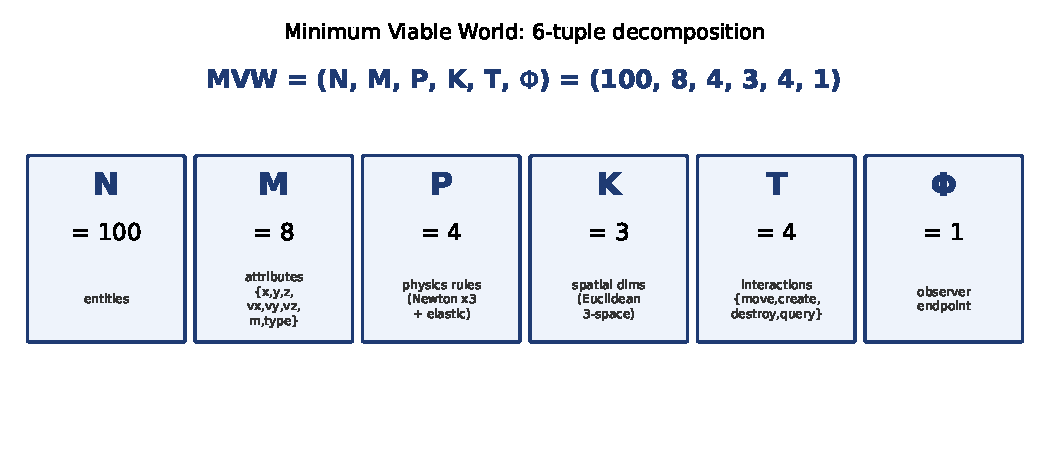
\includegraphics[width=0.92\textwidth]{figures/fig3_mvw_diagram.pdf}
\caption{The Minimum Viable World as a 6-tuple. Each parameter is the minimum
value satisfying the Tier C definition; $M$, $P$, $K$, and $\Phi$ are VERIFIED
from first principles, $T$ is PLAUSIBLE, and $N$ remains SPECULATIVE pending the
emergence-threshold question (Q1).}
\label{fig:mvw}
\end{figure*}

\subsection{Analytical Grounding for SCE-04}

The per-tick serial compute cost for MVW(100, 8, 4, 3, 4, 1) is bounded analytically.
State update requires $N \times M = 800$ operations per tick. Physics evaluation
requires $N \times P = 400$ operations per tick. Collision detection under a
naive all-pairs approach requires $\binom{N}{2} = 4{,}950$ comparisons per tick;
under a bounding volume hierarchy (BVH) \cite{ericson2004}, this reduces to
$O(N \log N) \approx 700$ operations at $N=100$.

The total per-tick cost is bounded:
\begin{equation}
    C_{\text{tick}} \leq 800 + 400 + 4{,}950 = 6{,}150 \text{ ops (naive)}
\end{equation}
\begin{equation}
    C_{\text{tick}} \leq 800 + 400 + 700 = 1{,}900 \text{ ops (BVH)}
\end{equation}

At $f_{\text{CPU}} = 1 \text{ GHz}$ (i.e., $10^9$ ops/sec), the achievable tick
rate far exceeds the 60 ticks/sec threshold:

\begin{equation}
    R_{\text{tick}} = \frac{10^9}{6{,}150} \approx 162{,}000 \text{ ticks/sec} \gg 60
\end{equation}

This provides analytical (though not empirical) grounding for SCE-04.

\subsection{Empirical Reference Implementation}

We implemented the MVW as a single-threaded, standard-library-only Python kernel
(world state, Newtonian physics with both naive $O(N^2)$ and BVH $O(N\log N)$
collision detection, a serial tick scheduler, and an observer interface). It
serves as the empirical counterpart to the analytical model and as the
system-under-test for the benchmark suite. Profiling on a single pinned core
yields the first empirical SCE results (Table~\ref{tab:sce-emp}).

\begin{table}[ht]
\caption{Empirical SCE results (CPython, single core)}
\label{tab:sce-emp}
\centering
\small
\begin{tabular}{p{0.8cm}p{4.4cm}p{2.2cm}}
\toprule
\textbf{ID} & \textbf{Measurement} & \textbf{Value} \\
\midrule
SCE-01 & Mean cost per tick (MVW, naive) & $\sim$3.25 ms \\
SCE-02 & RAM per entity & $\sim$393 bytes \\
SCE-03 & Scaling-law best fit (naive / BVH) & $O(N^2)$ / $O(N\log N)$ \\
SCE-04 & Sustained tick rate (60\,s, single core) & $\sim$311 ticks/sec \\
\bottomrule
\end{tabular}
\end{table}

SCE-04 passes with $\sim 5\times$ headroom over the 60 ticks/sec threshold. The
gap between this and the analytical $\sim$162{,}000 ticks/sec is the CPython
interpreter tax: each abstract ``operation'' in the analytical model maps to many
interpreter bytecodes. The measurement therefore corroborates the serial
sufficiency claim conservatively---a compiled serial implementation would
approach the analytical figure. SCE-03 empirically confirms the two scaling
regimes assumed above. Advancing SCE-04 to VERIFIED requires reproduction on the
declared serial-baseline hardware (a documented validation plan).

\subsection{Scaling Boundary}

Under the naive $O(N^2)$ collision model, serial sufficiency degrades when:
\begin{equation}
    \frac{10^9}{N^2/2} < 60 \implies N > \sqrt{\frac{10^9}{30}} \approx 5{,}774
\end{equation}

Under BVH ($O(N \log N)$), the boundary extends to approximately $N \approx 10^8$,
well beyond any practical MVW instantiation. The architectural choice of BVH
vs. naive collision detection is therefore load-bearing for the serial sufficiency
claim at larger $N$.

\begin{figure}[t]
\centering
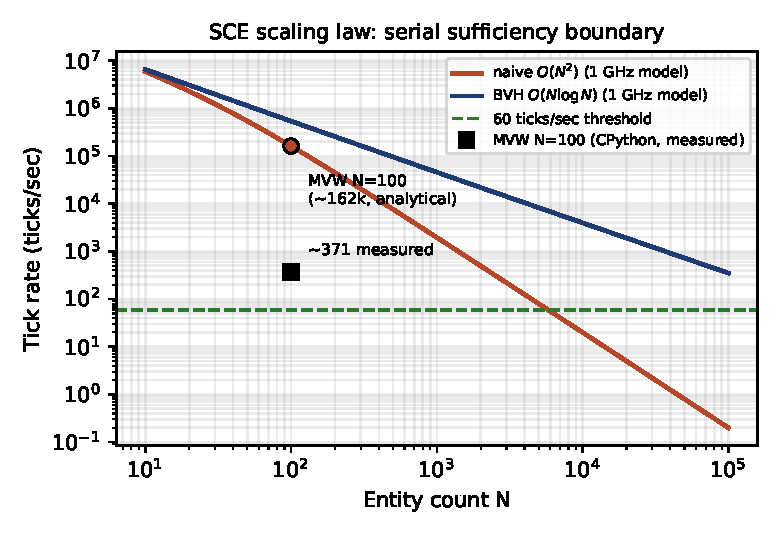
\includegraphics[width=\columnwidth]{figures/fig2_scaling_law.pdf}
\caption{SCE scaling law. The analytical 1\,GHz model places naive $O(N^2)$ and
BVH $O(N\log N)$ tick rates far above the 60 ticks/sec threshold at $N=100$; the
naive curve crosses the threshold near $N\approx5{,}774$. The black marker is the
empirical CPython reference measurement (\(\sim\)311 ticks/sec over a 60\,s
single-core run), which clears the threshold by \(\sim5\times\) despite a large
interpreter tax. A profiling sweep confirms the empirical fits: naive$=O(N^2)$,
BVH$=O(N\log N)$.}
\label{fig:scaling}
\end{figure}

%% ============================================================
\section{Adversarial Integrity Analysis}

We apply adversarial review to the benchmark framework itself, identifying five
classes of integrity failure.

\textbf{Attack 1 --- Circular Dependency (resolved):} Six benchmarks (TC-03,
SCE-01--04) referenced ``minimum viable world complexity'' without definition.
MVW (Section IV) resolves this dependency. Residual gap: $N=100$ threshold
is analytically motivated but not empirically calibrated (see Open Question Q1).

\textbf{Attack 2 --- Undecidable Benchmark (resolved):} PSF-04 originally required
``no undefined behavior'' across all interactions---a formally undecidable property
for open environments \cite{turing1936}. Replaced with closed interaction matrix
coverage requirement.

\textbf{Attack 3 --- Threshold Arbitrariness (partially resolved):} Thresholds
marked SPECULATIVE (WSI-03, TC-03, SCE-01, SCE-02, EG-03) lack empirical
calibration. SCE-04 receives analytical grounding via MVW (Section IV). Remaining
thresholds are documented as open calibration tasks.

\textbf{Attack 4 --- Floating Point Non-Determinism (addressed):} DR-01
cross-platform determinism is non-trivial because IEEE 754 behavior varies across
compiler optimizations and CPU architectures \cite{goldberg1991, monniaux2008}.
Investigation (Q3, Section~VI) reduces this to a single hazardous operation in the
kernel---now replaced by a portable cube root---and demonstrates a fixed-point
fallback that is bit-identical across platforms by construction.

\textbf{Attack 5 --- Missing Observer Domain (resolved):} The original seven
domains constituted a formally closed system with no external verification
mechanism. Domain 8 (Observer Interface) resolves this.

\textbf{Net integrity assessment:} 4 of 5 attacks fully resolved (the
floating-point strategy now addressed via Q3), 1 partially resolved (threshold
calibration, with SCE now empirically measured). The framework is structurally
sound and now backed by a reference implementation.

%% ============================================================
\section{Open Research Questions: Initial Results}

The four questions framed by this work were investigated with the reference
implementation. Three are now resolved and one is partially resolved with
empirical evidence; the experiments are reproducible from the repository.

\textbf{Q1 --- Minimum emergence threshold (partial):} We operationalized
``emergent behavior'' with three proxies. (i)~\textit{Thermalization}: starting
each particle at equal speed with random direction (each velocity component
Uniform, excess kurtosis $-1.2$), an isolated elastic gas relaxes toward the
microcanonical equilibrium, whose single-component excess kurtosis is exactly
$-6/(3N+2)$---Gaussian (the Maxwell--Boltzmann signature) only as
$N\to\infty$. Measured equilibrium kurtosis tracks this law
(Fig.~\ref{fig:q1}), giving a concrete threshold: the velocity distribution is
Gaussian to within $2\%$ at $N\approx 100$, within $5\%$ at $N\gtrsim 40$.
(ii)~\textit{Mixing}: a $10^{-6}$ perturbation diverges with positive Lyapunov
exponent for all $N\ge 2$---chaos is not the binding constraint.
(iii)~\textit{Interaction-onset}: at the nominal box $L=100$ the gas is
collision-starved ($\sim$0 collisions/particle at $N=100$). The binding
under-specification is therefore \textit{density}, not $N$: we recommend
promoting the MVW to a 7-tuple with an explicit packing fraction.
$N=100$ is supported as a statistical minimum.

\begin{figure}[t]
\centering
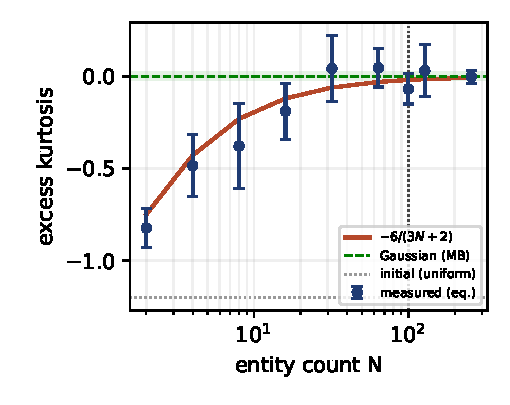
\includegraphics[width=0.82\columnwidth]{figures/fig4_q1_kurtosis.pdf}
\caption{Q1. Measured equilibrium velocity-component excess kurtosis vs.\ $N$
(fixed density) tracks the microcanonical law $-6/(3N+2)$, rising from the
non-equilibrium initial value ($-1.2$) into the $\pm2\%$ Gaussian
(Maxwell--Boltzmann) band near $N=100$.}
\label{fig:q1}
\end{figure}

\textbf{Q2 --- BVH serial classification (resolved):} The reference BVH build and
traversal run in a single thread and are deterministic; the median-split
construction has measured log--log time-scaling exponent $\approx 1.12$
($O(N\log N)$) versus $\approx 2.06$ for the naive scan. An independent serial
broad-phase (sweep-and-prune) and the naive scan return identical overlap sets,
so serial spatial indexing is not unique to BVH. Under Interpretation 1 the BVH
\textit{counts as serial}: it does not require parallelism, and the Section~IV
scaling analysis holds.

\textbf{Q3 --- Fixed-point vs. IEEE 754 (resolved):} A static audit shows the
kernel hot path uses only correctly-rounded IEEE-754 operations
($+,-,\times,\div,\sqrt{\ }$), which are bit-portable; the sole cross-platform
hazard is the cube-root \texttt{pow} used once per entity for the collision
radius, now replaced by a portable Newton-based cube root. Independently, a
pure-integer fixed-point elastic-collision solver---bit-identical across
platforms by construction---preserves momentum conservation to within $10^{-6}$
(the PSF-02 threshold) at scale factor $S\ge 2^{26}$, with error scaling as
$1/S$. Cross-platform determinism is thus achievable either way.

\textbf{Q4 --- Turing completeness of interaction vocabulary (resolved):} The
subset $\{\text{create, destroy, query}\}$ is Turing-complete by reduction to a
Minsky register machine \cite{minsky1967}: a register is the population of an
entity type, with $\text{INC}=\text{create}$, $\text{DEC}=\text{query}{+}\text{destroy}$,
and $\text{JZ}=\text{query-for-zero}$. We confirmed this empirically by storing
all machine state in an MVW world and executing register-machine programs
(addition and multiplication, the latter with nested loops) through the
interaction vocabulary alone; all returned correct results. The vocabulary is
universal under query-conditioned control; \texttt{move} adds spatial
expressiveness, not computational power, so $T=4$ is sufficient (and not minimal)
for the ``arbitrary environment'' claim of EG-01.

%% ============================================================
\section{Conclusion}

We have presented a benchmark framework for holodeck-class simulation systems
grounded in serial compute foundations, comprising eight domains, a formal
Minimum Viable World definition, and a single-threaded standard-library reference
implementation. An adversarial integrity analysis resolved four of five
identified failures, the last (floating-point determinism) addressed through the
research questions below.

The serial sufficiency claim is supported both analytically and empirically. The
analytical model gives $\sim$162{,}000 ticks/sec for a 100-entity Newtonian
simulation at 1 GHz; the CPython reference engine sustains $\sim$311 ticks/sec on
a single core---still $\sim 5\times$ over the 60 ticks/sec threshold, the gap
being interpreter overhead rather than an architectural limit. Advancing SCE-04
from measured to formally VERIFIED requires reproduction on the declared
serial-baseline hardware.

The four research questions originally posed as open are now substantially
answered: the emergent Maxwell--Boltzmann velocity distribution is Gaussian to
within $2\%$ near $N=100$ (with spatial density, not $N$, identified as the
binding parameter); the bounding-volume hierarchy is serial-compatible; both a
portable cube root and a fixed-point fallback secure cross-platform determinism;
and the interaction vocabulary is Turing-complete via a register-machine
reduction verified in the reference engine. Three of the four are resolved; Q1
remains partially open on density calibration.

The benchmark set, reference implementation, and reproducible experiments are
available as an open repository to support community validation efforts.

%% ============================================================
\bibliographystyle{IEEEtran}
\bibliography{references}

\end{document}
